\documentclass{article}
\usepackage[utf8]{inputenc}
\usepackage{polski}
\usepackage[polish]{babel}
\usepackage{bbm}
\usepackage{amsmath}
\usepackage{amsthm}
\usepackage{graphicx}
\usepackage{epstopdf}
\usepackage[export]{adjustbox}
\usepackage{float}

\newtheorem{defi}{Definicja}
\newtheorem{twr}{Twierdzenie}
\newtheorem*{dd}{Dowód}

\DeclareMathOperator{\sign}{sign}
\DeclareMathOperator{\arctg}{arctg}

\newcommand{\twopartdef}[4]
{
	\left\{
		\begin{array}{ll}
			#1 & \mbox{jeśli } #2 \\
			#3 & \mbox{jeśli } #4
		\end{array}
	\right.
}


\author{Jarosław Dzikowski 273233}
\date{Wrocław, \today}
\title{\textbf{Bazy danych} \\ Rowery miejskie - model konceptualny}
\begin{document}
\maketitle

\section{Diagram E-R}
Diagram E-R został zamieszczony na osobnej stronie ze względu na swoją wielkość.
\pagenumbering{gobble}% Remove page numbers (and reset to 1)
%\clearpage
\begin{figure}[p]
\centerline{	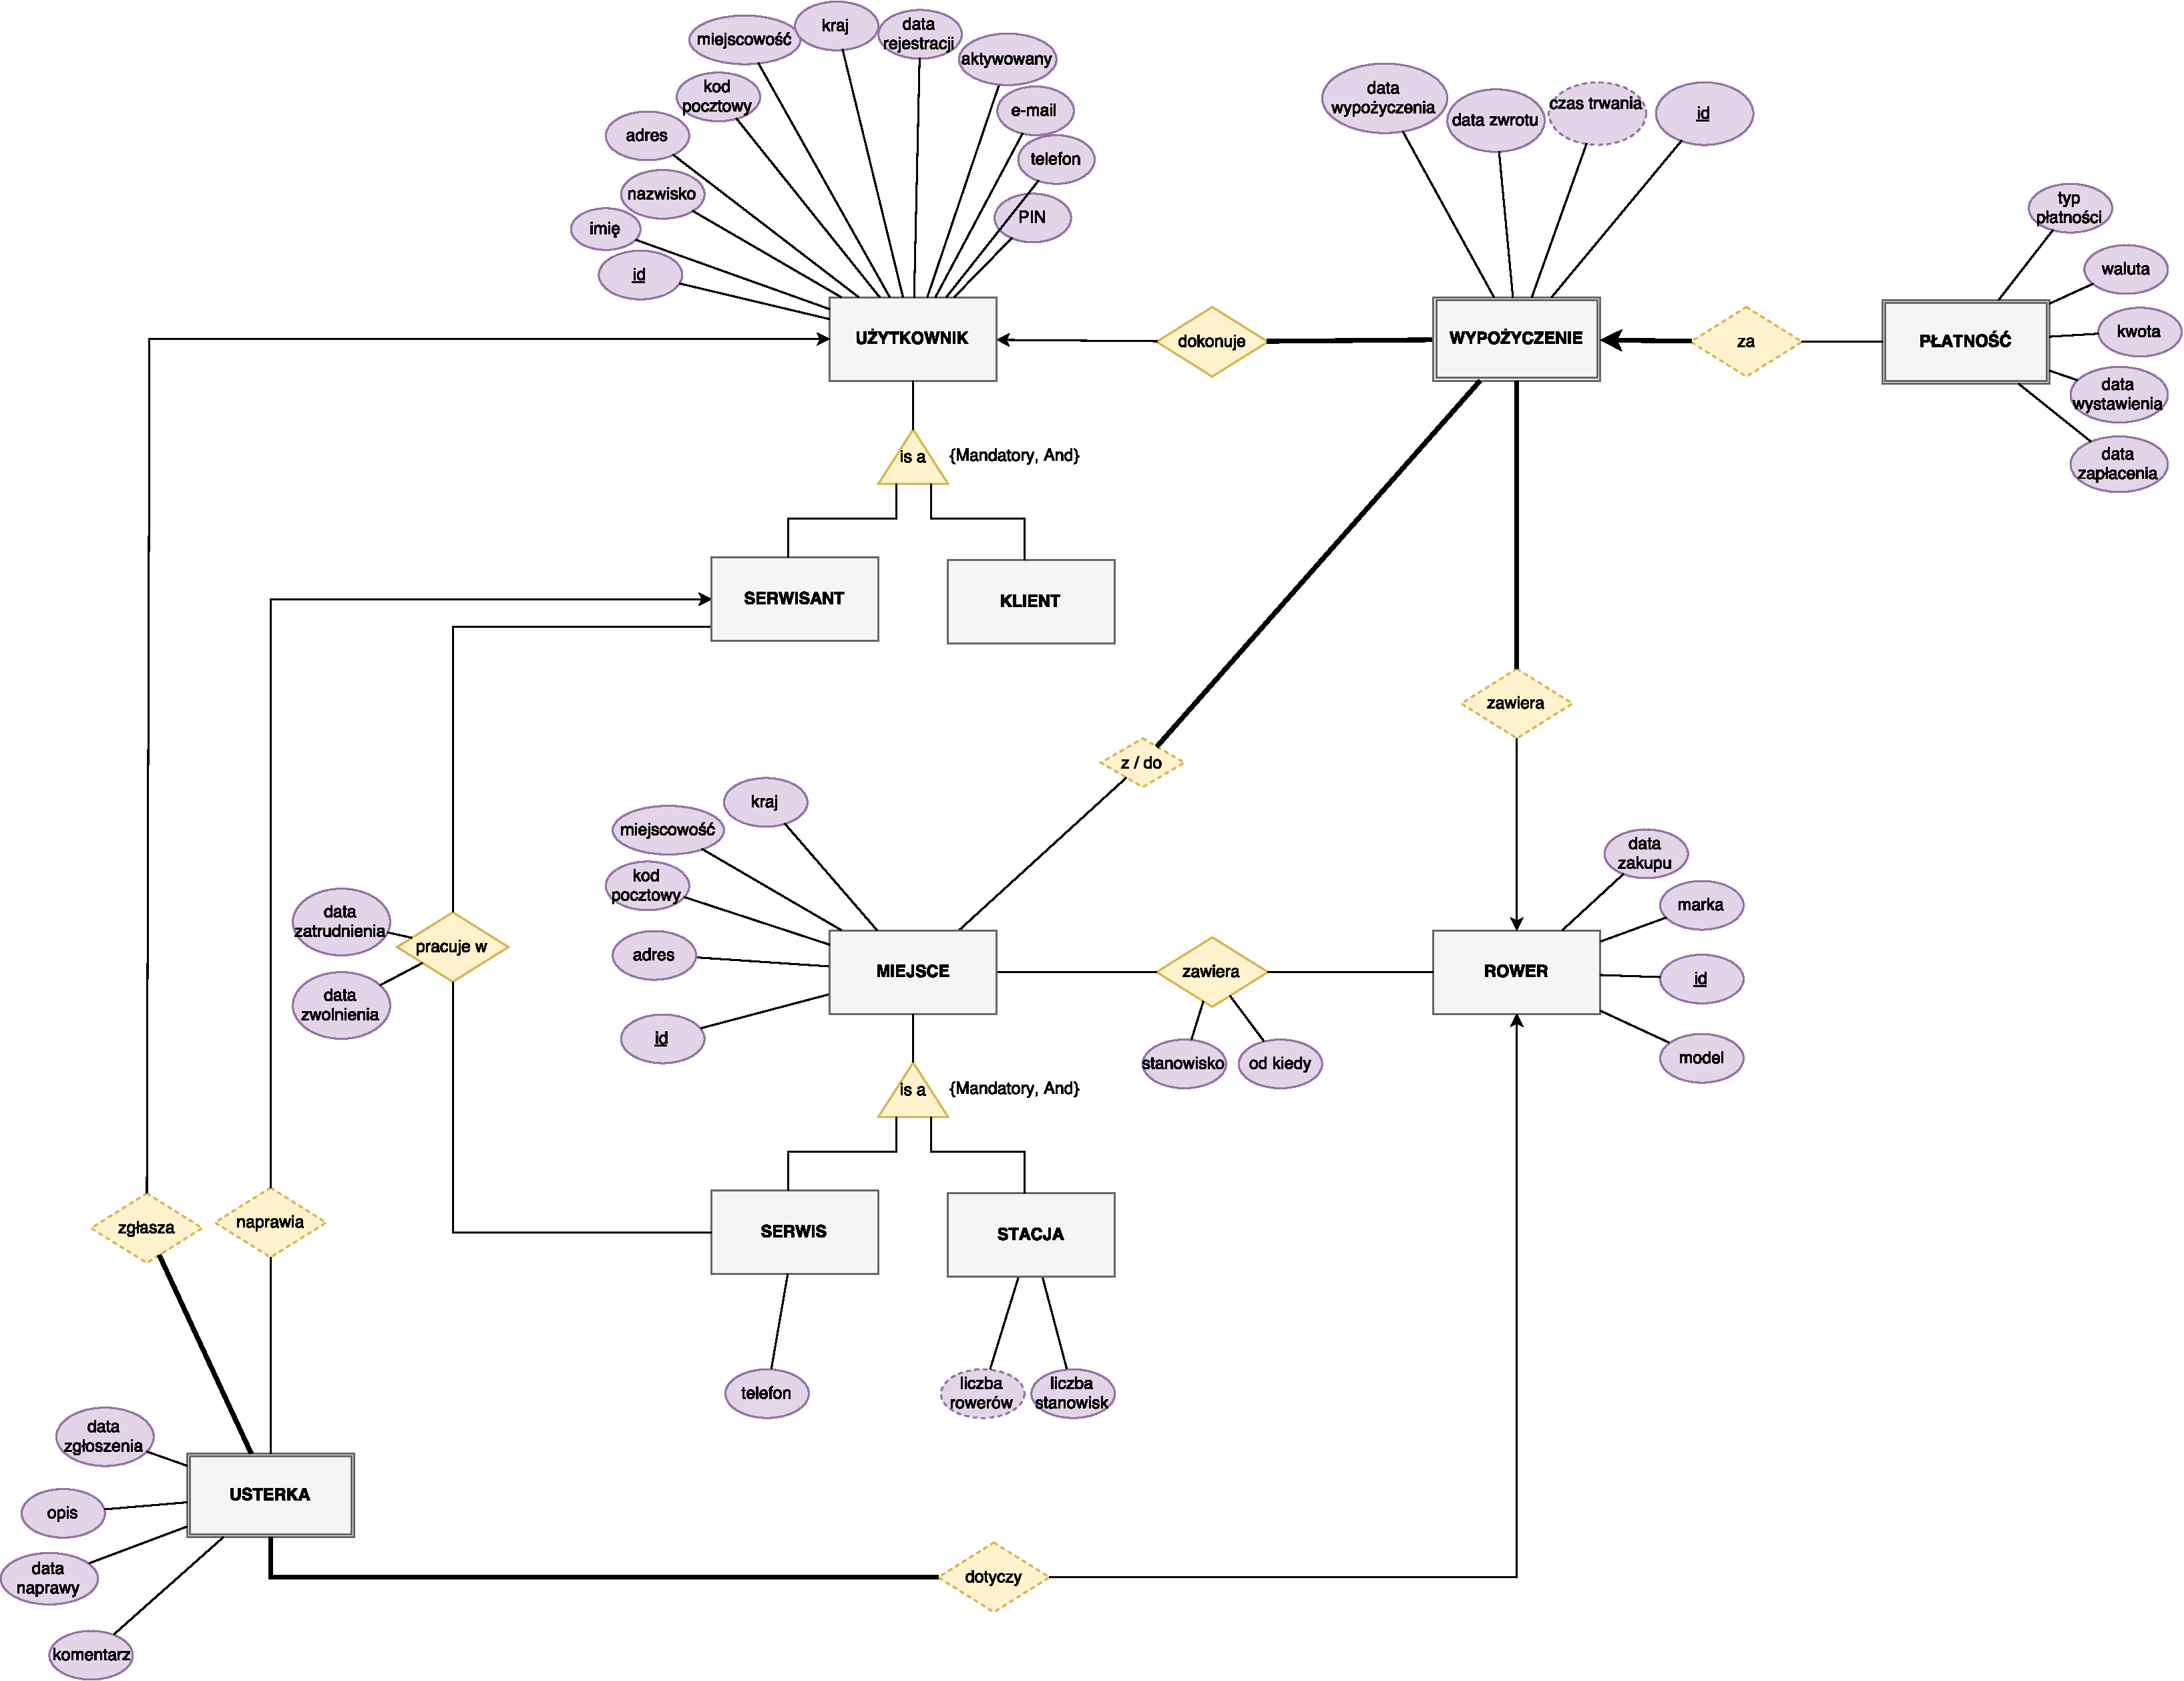
\includegraphics[width=\paperwidth, height=\paperheight, keepaspectratio]{diagramfinal.pdf}}
\end{figure}

\section{Komentarz}
Na diagramie widnieje dziesięć encji.
Cztery z nich są oczywiste z punktu widzenia zagadnienia rowerów miejskich.
Mamy użytkowników, rowery, miejsca oraz wypożyczenia.
Użytkownicy mogą być jednym z dwóch typów: klientem lub serwisantem. Mimo że na diagramie użytkownik
ma atrybut PIN, to tak naprawdę nie będziemy tego hasła pamiętać. Więcej o tym pod koniec tej sekcji.
Tak samo miejsca mogą być jednym z dwóch typów: stacją lub serwisem.
Oczywiście stacje i serwisy mają swoje własne charakterystyczne cechy takie jak liczba stanowisk
na stacji bądź telefon do serwisu.
Serwisanci pracują w serwisach - interesują nas daty zatrudnienia oraz zwolnienia,
ta druga może być nieznana, jesli serwisant dalej pracuje w danym serwisie.
Dopuszczamy pracę serwisanta w wielu serwisach, serwisant mógłby zostać wypożyczony do innego serwisu.
\newline
\newline
Użytkownicy dokonują wypożyczeń, które obejmują rowery (1 rower na wypożyczenie)
oraz 2 miejsca (początkowe i końcowe) a także stanowiska początkowe oraz końcowe.
Wypożyczenie obejmuje dwie sytuacje: wypożyczenie roweru przez klienta oraz przewiezienie roweru przez serwisanta.
Miejsca docelowe i końcowe mogą być albo serwisem albo stacją,
klient oczywiście będzie wypożyczał i zwracał rowery ze stacji, natomiast serwisant nie ma takiego ograniczenia.
Gdy jednym z miejsc wypożyczenia jest serwis,
to stanowisko nie ma wówczas żadnego znaczenia (W serwisach nie ma stanowisk z tego, co wiem).
\newline
\newline
Rowery znajdują się albo na stacjach, albo są wypożyczone, albo znajdują się w serwisie
(Na diagramie relacja Rower-Miejsce).
Za wypożyczenia naliczane są płatności, które zostały przedstawione jako kolejna encja.
Księgowy zajmujący się płatnościami może nakładać płatności
związane z trzema źródłami: wypożyczeniem, rejestracją, karą.
Wypożyczenie w płatności może być nullem, jeśli płatność dotyczy rejestracji.
\newline
\newline
Dodatkowo, zgłaszane są usterki przez użytkowników, które są naprawiane przez serwisantów.
Każda taka usterka posiada opis usterki oraz komentarz serwisanta/ów, którzy zajmowali się tą usterką.
\newline
\newline
\textbf{Uwaga:} W modelu fizycznym jest więcej tabel, widoków etc niż widać na tym diagramie.
Nie zostały one umieszczone, ponieważ nie są one ważne z punktu widzenia umodelowania zagadnienia rowerów miejskich.
Przykładem mógłby być sposób uwierzytelniania użytkowników. Loginem jest telefon, PIN jest hasłem, lecz w bazie danych
pamiętamy tak naprawdę losowy salt oraz hash skonkatenowanego salt'a z PINem podanym przez użytkownika. 
\newline
\newline
Nieopisane więzy są całkiem oczywiste, nie znalazłem żadnych bardziej skomplikowanych więzów:
\begin{enumerate}
	\item Liczba stanowisk na stacji musi być nieujemna.
	\item Data zwolnienia serwisanta musi być nie wcześniejsza niż data zatrudnienia.
	\item Rower może być tylko na nieujemnym stanowisku (Na stacji).
	\item Stanowiska z których wypożyczono oraz do których zwrócono rowery muszą być albo NULL albo nieujemne.
	\item Czas zwrotu roweru musi być nie wcześniejsze niż czas wypożyczenia roweru.
	\item Kwota naliczona w płatności musi być nieujemna.
	\item Data pokrycia płatności musi być nie wcześniejsza niż data jej wystawienia.
	\item Data naprawy usterki musi być nie wcześniejsza niż data jej zgłoszenia.
\end{enumerate}

\section{Opis ról}
\subsection{Rola klienta}
\begin{enumerate}
	\item Może dodawać nowe wypożyczenia i aktualizować swoje wypożyczenie.
	\item Prawo do wglądu do historii wypożyczeń.
	\item Prawo do wglądu do historii płatności.
	\item Może zobaczyć, gdzie są stacje.
	\item Może dodawać nowe usterki.
\end{enumerate}

\subsection{Rola serwisanta}
\begin{enumerate}
	\item Może dodawać nowe usterki i aktualizować stare.
	\item Prawo do wglądu do historii usterek.
	\item Może naprawiać usterki.
	\item Może przewozić rowery (Między stacjami i serwisami).
	\item Może sprawdzać, gdzie są rowery.
	\item Może sprawdzać, ile rowerów jest na której stacji.
	\item Może przeglądać katalog rowerów oraz dodawać nowe.
	\item Może przeglądać katalog stacji oraz serwisów.
\end{enumerate}

\subsection{Rola księgowego}
\begin{enumerate}
	\item Ma prawo do modyfikacji oraz odczytu danych płatności.
	\item Ma prawo do odczytu historii wypożyczeń.
	\item Ma prawo do odczytu danych użytkowników i aktywowania/dezaktywowania użytkowników.
	\item Nakłada płatności na użytkowników.
	\item Znajduje wypożyczenia z brakiem zwrotu roweru i nakłada kary na użytkowników wypożyczających.
\end{enumerate}

\end{document}
